\documentclass[12pt]{article}

% Packages
\usepackage[utf8]{inputenc}         % UTF-8 encoding
\usepackage{amsmath}                % Math symbols
\usepackage{graphicx}               % For including images
\usepackage{geometry}               % Page layout
\usepackage{caption}                % Better captions
\usepackage[hidelinks]{hyperref}    % Hyperlinks in the document
\usepackage{xcolor}
\usepackage{float}
\geometry{a4paper, margin=1in}      % Set margins

% Title Page
\title{Informe práctica: \textit{Métodos Variacionales}}
\author{Nicolás de Pineda Gutiérrez \\[1ex] 
\small Universidad de Sevilla}
\date{}
\begin{document}

\maketitle
\thispagestyle{empty}

\renewcommand{\contentsname}{Contenido}
\newpage
\tableofcontents 

\newpage
\section{Introducción}

En la primera parte, se van a estudiar propiedades físicas de isómeros con estaño a partir de simulaciones ab-initio.

La comparación de propiedades de isómeros a partir de simulaciones no es trivial, ya que las diferencias en energía entre isómeros son muy pequeñas, y al tomar una diferencia de dos números muy cercanos se pueden obtener errores significativos. Las diferencias de energía entre los isómeros estudiados son alrededor de 5 ordenes de magnitud más pequeñas que la energía total de los sistemas, por lo que se requiere de una precisión muy alta en los cálculos para que los resultados tengan sentido.

Para los cálculos teóricos, se utilizará el método Hartree-Fock (HF), un método variacional, optimizando los orbitales moleculares como combinación lineal de las bases, para minimizar la energía total del sistema. El resultado de estos cálculos será aproximado, ya que el limite Hartree-Fock no incluye correlación electrónica completa. Además, la cercanía del calculo al límite Hartree-Fock, dependerá de la base utilizada. 

Se usarán las bases LANL2DZ y SDD, que son bases de pseudopotencial, o ECP (effective core potential), que permiten acelerar los cálculos al reemplazar los electrones internos por un potencial efectivo, y reducir el número de orbitales a calcular. Sin embargo, estas bases no añaden orbitales de polarización, para átomos pequeños, por lo que los cálculos, no tendrán una buena calidad para la parte no-ECP. La parte no-ECP se corresponde a los átomos menos pesados que el sodio para LANL2DZ (en nuestros compuestos: H, C, F), y menos pesados que el potasio para SDD (H, C, F, Cl), lo que significa, que es probable que estos cálculos no estén cerca del límite Hartree-Fock. Para la parte que no utiliza potenciales de core efectivos, y se optimizan todos los orbitales, las bases LANL2DZ y SDD son equivalentes a una base 6-31G \cite{batista_gaussian}. Por esta razón, estas bases son generalmente mejores para complejos inorgánicos, que para compuestos orgánicos, ya que los orbitales de polarización son importantes para describir la carga de los átomos en moléculas polares.

Para átomos pesados como el estaño, se necesitan tomar en cuenta efectos relativistas para obtener resultados precisos. Estos efectos están parcialmente añadidos por el uso de las bases de pseudopotencial SDD y LANL2DZ.

En la segunda parte, se estudiarán propiedades de compuestos $M^{2+}-C_6H_6$, donde M=Be, Mg, Ca y Sr, para estudiar la influencia del tamaño del átomo en las propiedades del compuesto, como la distancia de enlace, la carga del metal, y la frecuencia de vibración del enlace metal-anillo. Además se estudiará el cambio en las propiedades al añadir orbitales $d$ difusos a la base.



% \section{Isomeros del clorofluorobutadieno}
%
% \subsection{Cargas de Mulliken}
% \begin{center}
%     \begin{tabular}{|r|c|c|c|c|c|c|c|}
%         \multicolumn{8}{c}{\textbf{Cargas de Mulliken (Isómero 1)}} \\
%         \hline
%         Method      & $q_{C1}$ & $q_{C2}$ & $q_{C3}$ & $q_{C4}$ & $q_{F}$  & $q_{Cl}$ & $\mu (D)$  \\
%         \hline
%         6-31G       & 0.141 & -0.199 & -0.142 & -0.362 & -0.403 & 0.148  & 2.883 \\
%         6-31G(d)    & 0.302 & -0.258 & -0.143 & -0.403 & -0.340 & 0.022  & 1.799 \\
%         6-31G(d, p) & 0.292 & -0.192 & -0.104 & -0.290 & -0.339 & 0.022  & 1.793 \\
%         cc-pVDZ     & 0.239 & -0.022 & -0.090 & -0.005 & -0.235 & -0.079 & 1.711 \\
%         cc-pVTZ     & 0.307 & -0.217 & -0.087 & -0.339 & -0.195 & -0.111 & 1.579 \\
%         cc-pVQZ     & 0.354 & -0.281 & -0.170 & -0.216 & -0.257 & -0.027 & 1.593 \\
%         \hline
%     \end{tabular}
% \end{center}
%
% \begin{center}
%     \begin{tabular}{|r|c|c|c|c|c|c|c|}
%         \multicolumn{8}{c}{\textbf{Cargas de Mulliken (Isómero 3)}} \\
%         \hline
%         Method       & $q_{C1}$ & $q_{C2}$ & $q_{C3}$ & $q_{C4}$ & $q_{F}$ & $q_{Cl}$ & $\mu (D)$ \\
%         \hline
%         6-31G       & -0.531 & 0.552 & -0.187 & -0.340 & -0.436 & 0.085  & 3.746 \\
%         6-31G(d)    & -0.439 & 0.539 & -0.218 & -0.386 & -0.366 & 0.003  & 2.930 \\
%         6-31G(d, p) & -0.375 & 0.522 & -0.171 & -0.272 & -0.366 & 0.002  & 2.939 \\
%         cc-pVDZ     & -0.170 & 0.396 & -0.164 & 0.017  & -0.255 & -0.070 & 2.832 \\
%         cc-pVTZ     & -0.194 & 0.341 & -0.173 & -0.317 & -0.205 & -0.120 & 2.703 \\
%         \hline
%     \end{tabular}
% \end{center}
%
%
% \subsection{Energías relativas}
%
%
% \begin {center}
%         \begin{tabular}{|c|r|r|r|r|r|}
%         \multicolumn{6}{c}{\textbf{Energías totales (Hartree)}} \\
%         \hline
%         Isomero & 6-31G & 6-31G(d) & 6-31G(d,p) & cc-pVDZ & cc-pVTZ \\
%         \hline
%         (1) & -712.553355 & -712.664593 & -712.671792 & -712.705559 & -712.799431 \\
%         (2) & -712.561125 & -712.668188 & -712.675375 & -712.708841 & -712.801187 \\
%         (3) & -712.560978 & -712.669540 & -712.676705 & -712.709783 & -712.802547 \\
%         (4) & -712.554082 & -712.665845 & -712.673015 & -712.706839 & -712.800219 \\
%         (5) & -712.557569 & -712.663762 & -712.671167 & -712.704918 & -712.797424 \\
%         (6) & -712.555559 & -712.663176 & -712.670593 & -712.704027 & -712.797440 \\
%         \hline
%     \end{tabular}
% \end{center}
%
%
%
%
% \subsection{Frecuencias de vibración}
%
% \begin{center}
%     \begin{tabular}{|r|c|c|c|c|}
%         \multicolumn{5}{c}{\textbf{Frecuencias de vibración ($\mathbf{cm^{-1}}$) (Isómero 1) }} \\
%         \hline
%         Base & $\nu_{C-H}$ & $\nu_{C=C}$ & $\nu_{C-F}$ & $\nu_{C-Cl}$ \\
%         \hline
%         6-31G       & 3425-3333 & 1934, 1838 & 1225 & 718 \\
%         6-31G(d)    &  &  &  &  \\
%         6-31G(d, p) &  &  &  &  \\
%         cc-pVDZ     &  &  &  &  \\
%         cc-pVTZ     &  &  &  &  \\
%         \hline
%     \end{tabular}
% \end{center}
%
%
%
% \begin{center}
%     \begin{tabular}{|r|c|c|c|c|}
%         \multicolumn{5}{c}{\textbf{Frecuencias de vibración ($\mathbf{cm^{-1}}$) (Isómero 3) }} \\
%         \hline
%         Base & $\nu_{C-H}$ & $\nu_{C=C}$ & $\nu_{C-F}$ & $\nu_{C-Cl}$ \\
%         \hline
%         6-31G       &  &  &  &  \\
%         6-31G(d)    &  &  &  &  \\
%         6-31G(d, p) &  &  &  &  \\
%         cc-pVDZ     &  &  &  &  \\
%         cc-pVTZ     &  &  &  &  \\
%         \hline
%     \end{tabular}
% \end{center}
%
%
% \subsection{Distancias de enlace}
% \begin{center}
%     \begin{tabular}{|r|c|c|c|c|}
%         \multicolumn{5}{c}{\textbf{Frecuencias de vibración ($\mathbf{cm^{-1}}$) (Isómero 3) }} \\
%         \hline
%         Method      & $r_{F-C}$ & $r_{Cl-C}$ & $r_{H-C}$ & $r_{C=C}$ \\
%         \hline
%         6-31G       & 1.361 & 1.775 & 1.073 & 1.320 \\
%         6-31G(d)    & 1.318 & 1.718 & 1.075 & 1.318 \\
%         6-31G(d, p) & 1.318 & 1.718 & 1.076 & 1.318 \\
%         cc-pVDZ     & 1.316 & 1.722 & 1.083 & 1.321 \\
%         cc-pVTZ     & 1.309 & 1.716 & 1.074 & 1.315 \\
%         \hline
%     \end{tabular}
% \end{center}






\definecolor{r}{rgb}{0.8, 0.2, 0.2}
\newcommand{\low}{\textcolor{r}{0.00}}
\section{Estudio de isómeros del (fluorobromovinil)diestaneno}
\begin{center}
    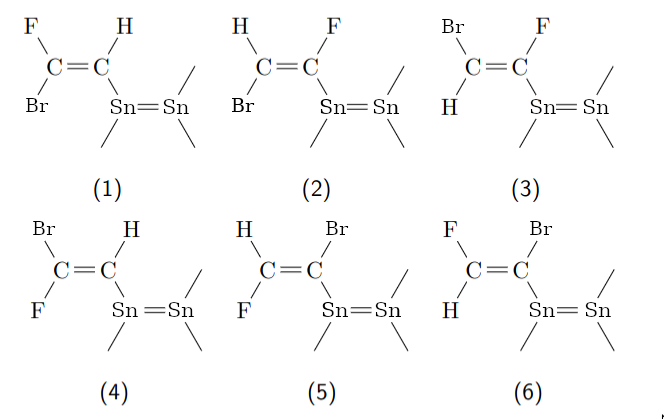
\includegraphics[height=0.35\textwidth]{isomers_sn.png}
    \captionof{figure}{Isómeros a estudiar.}
\end{center}

\subsection{Energías relativas}

Se obtienen las energías RHF de los isómeros usando distintos métodos. Se utilizan dos bases, LANL2DZ y SDD. Los resultados se muestran en la tabla 1. 

\begin{table}[H]
\centering
\begin{tabular}{ccccc}
\hline
    Isómero & \text{HF/LANL2DZ} & \text{HF/SDD} \\
\hline
    (1) & -196.781975 & -196.997451 \\
    (2) & -196.785238 & -197.000700 \\
    (3) & -196.788565 & -197.004545 \\
    (4) & -196.786164 & -197.001948 \\
    (5) & -196.789361 & -197.004664 \\
    (6) & -196.789456 & -197.004741 \\
\hline
\end{tabular}
\caption{Energías (Hartree)}
\end{table}

A partir de las energías obtenidas se calculan las diferencias de energía entre los isómeros, y el isómero de menor energía, que se muestran en la tabla 2.

\begin{table}[H]
\centering
\begin{tabular}{ccccc}
\hline
    Isómero & \text{HF/LANL2DZ} & \text{HF/SDD} \\
\hline
    (1) &9.64 & 19.14 \\
    (2) &1.08 & 10.61 \\
    (3) &0.34 & 0.51  \\
    (4) &0.64 & 7.33  \\
    (5) &0.25 & 0.20  \\
    (6) &\low & \low  \\
\hline
\end{tabular}
\caption{Diferencias de energía (kJ/mol)}
\end{table}

Se observa que las diferencias de energía entre isómeros son muy pequeñas. 

El isómero más estable, es el isómero 6, que a su vez tiene una estabilidad muy cercana al isómero 3 y 5, para la base SDD, y también al 4 y 2, para la base LANL2DZ. 

Comparándola con energías relativas de isómeros sin estaño:
\begin{center}
    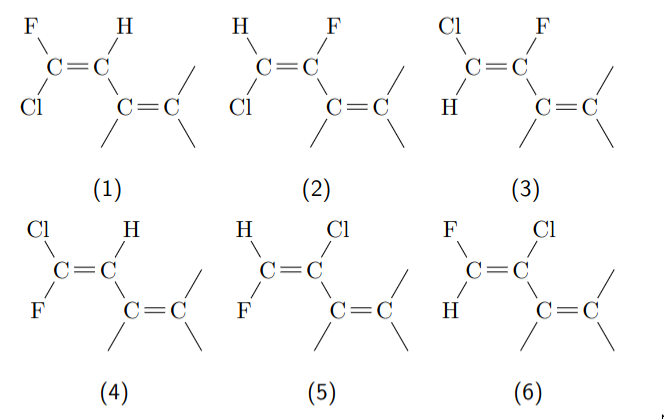
\includegraphics[height=0.35\textwidth]{isomers.png}
    \captionof{figure}{Isómeros sin estaño.}
\end{center}
\begin{table}[H]
\centering
\begin{tabular}{cccccc}
    \hline
    Isómero & 6-31G & 6-31G(d) & 6-31G(d,p) & cc-pVDZ & cc-pVTZ \\
    \hline
    (1) & 20.40 & 12.99 & 12.90 & 11.09 & 8.18 \\
    (2) & \low & 3.55 & 3.49 & 2.47 & 3.57 \\
    (3) & 0.39 & \low & \low & \low & \low \\
    (4) & 18.49 & 9.70 & 9.69 & 7.73 & 6.11 \\
    (5) & 9.34 & 15.17 & 14.54 & 12.77 & 13.45 \\
    (6) & 14.61 & 16.71 & 16.05 & 15.11 & 13.41 \\
    \hline
\end{tabular}
\caption{Diferencias de energía de isómeros sin estaño (kJ/mol)}
\end{table}

El isómero de menor energía, para todas las bases menos la 6-31G, es el 3. Además, la diferencia de energía entre el isómero 2 y 3 para la base 6-31G es de 0.39 kJ/mol, especialmente pequeña, por lo que no parece que se pierda demasiada información cualitativa al usar bases sin funciones de polarización.

No se observa ninguna correlación entre que isómero es más estable con o sin el estaño, lo que sugiere que el estaño tiene un efecto significativo en la estabilidad de los isómeros.


Algo notable de estas estructuras, que se puede observar a partir de estas optimizaciones, es que no se trata de estructuras planas, como se podría esperar de un compuesto con enlaces dobles, sino que la molécula distorsionada tiene una menor energía que la molécula plana. \cite{marquez_sn2h4} 

\begin{center}
    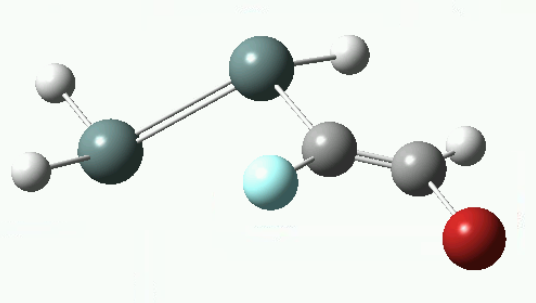
\includegraphics[height=0.30\textwidth]{3d.png}
    \captionof{figure}{Estructura 3D del Isómero 3.}
\end{center}


% \begin {center}
%     \begin{tabular}{|c|r|c|c|c|c|}
%         \multicolumn{6}{c}{\textbf{Diferencias de energías relativas (kJ/mol)}} \\
%         \hline
%         Isomero & 6-31G & 6-31G(d) & 6-31G(d,p) & cc-pVDZ & cc-pVTZ \\
%         \hline
%         (1) & 20.4 & 12.1 & 12.9 & 11.1 & 8.2  \\
%         (2) & \low & 3.6  & 3.5  & 2.5  & 3.6  \\
%         (3) & 0.4  & \low & \low & \low & \low  \\
%         (4) & 18.5 & 9.7  & 9.7  & 7.7  & 6.1  \\
%         (5) & 9.3  & 15.2 & 14.5 & 12.8 & 13.5 \\
%         (6) & 14.6 & 16.7 & 16.1 & 15.1 & 13.4 \\
%         \hline
%     \end{tabular}
% \end {center}






\newpage
\subsection{Cargas de Mulliken}

\begin{table}[H]
\centering
    \begin{tabular}{rcccccc}
        \hline
        Base & $q_{C_1}$ & $q_{C_2}$ & $q_{Sn_1}$ & $q_{S_n2}$ & $q_{Br}$ & $q_{F}$ \\
        \hline
        HF/LANL2DZ  & 0.164 & -0.563 & 0.632 & 0.350 & 0.042 & -0.314 \\
        HF/SDD      & 0.165 & -0.577 & 0.587 & 0.345 & 0.077 & -0.315 \\
        \hline
    \end{tabular}
    \caption{Cargas de Mulliken del Isómero 1}
\end{table}

\begin{table}[H]
\centering
    \begin{tabular}{rcccccc}
        \hline
        Base & $q_{C_1}$ & $q_{C_2}$ & $q_{Sn_1}$ & $q_{Sn_2}$ & $q_{Br}$ & $q_{F}$ \\
        \hline
        HF/LANL2DZ  & 0.473 & 0.086 & 0.594 & 0.427 & 0.027 & -0.355 \\
        HF/SDD      & 0.496 & 0.090 & 0.561 & 0.415 & 0.067 & -0.357 \\
        \hline
    \end{tabular}
    \caption{Cargas de Mulliken del Isómero 3}
\end{table}

El flúor, al ser más electronegativo, tiene una carga negativa, mientras que el bromo, es prácticamente neutro. Los carbonos y estaños tienen cargas positivas, siendo los átomos más electropositivos, junto con el hidrógeno. Es posible que si se añadieran orbitales de polarización a la base, las cargas de los átomos más electronegativos cambiaran significativamente, ganando el bromo una carga negativa, y reduciéndose la carga negativa del flúor.

Las cargas no varían significativamente entre los isómeros, y son similares entre las bases utilizadas. Esto puede deberse a que ninguna de las bases utilizadas añade orbitales de polarización, que son importantes para describir la carga de los átomos en moléculas polares. Estas bases corresponden a bases 6-31G\cite{batista_gaussian}, pero usando potencial efectivo y añadiendo correcciones relativistas.

Comparándolo con resultados de cálculos HF, pero son de compuestos sin estaño:
\begin{center}
    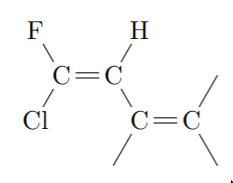
\includegraphics[height=0.14\textwidth]{ISO1.png}
    \captionof{figure}{Compuesto sin estaño.}
\end{center}


\begin{table}[H]
\centering
    \begin{tabular}{rcccccc}
        \hline
        Base & $q_{C_1}$ & $q_{C_2}$ & $q_{C_3}$ & $q_{C_4}$ & $q_{F}$ & $q_{Cl}$ \\
        \hline
        6-31G      & 0.141 & -0.199 & -0.142 & -0.362 & -0.403 & 0.148 \\
        6-31G(d)   & 0.303 & -0.258 & -0.143 & -0.403 & -0.340 & 0.022 \\
        6-31G(d,p) & 0.292 & -0.192 & -0.104 & -0.290 & -0.339 & 0.022 \\
        cc-pVDZ    & 0.239 & -0.022 & -0.090 & -0.005 & -0.235 & -0.079 \\
        cc-pVTZ    & 0.307 & -0.217 & -0.087 & -0.339 & -0.195 & -0.111 \\
        \hline
    \end{tabular}
    \caption{Cargas de Mulliken del compuesto sin estaño}
\end{table}

Las cargas varían significativamente al añadir orbitales de polarización a la base.

También podemos observar que el estaño, al ser mucho más electropositivo que el carbono, tiene una carga positiva significativa, al contrario que el $C_3$ y $C_4$ de los compuestos sin estaño, que tienen cargas negativas, algo que afecta a la distribución de cargas de la molécula.






\subsection{Distancias de enlace}
\begin{table}[H]
\centering
    \begin{tabular}{rcccccc}
        \hline
        Base & C-F & C-Br & C-H & C=C & Sn=Sn & Sn-C \\
        \hline
        HF/LANL2DZ  & 1.378 & 1.927 & 1.080 & 1.320 & 2.789 & 2.139 \\
        HF/SDD      & 1.378 & 1.918 & 1.080 & 1.320 & 2.785 & 2.163 \\
        \hline
    \end{tabular}
    \caption{Distancias (Isómero 1) (Ángstrom)}
\end{table}

\begin{table}[H]
\centering
    \begin{tabular}{rcccccc}
        \hline
        Base & C-F & C-Br & C-H & C=C & Sn=Sn & Sn-C \\
        \hline
        HF/LANL2DZ   & 1.397 & 1.939 & 1.068 & 1.326 & 2.817 & 2.163 \\
        HF/SDD       & 1.396 & 1.928 & 1.068 & 1.326 & 2.813 & 2.186 \\
        \hline
    \end{tabular}
    \caption{Distancias (Isómero 3) (Ángstrom)}
\end{table}
Para distancias como la C-H, que hay multiples, se da la distancia media.

La distancia de enlace C=C del isómero 1, es ligeramente menor que la del isómero 3, que se puede explicar por la diferencia de cargas entre los carbonos. En el isómero 1, los carbonos tienen cargas opuestas, por lo que se atraen ligeramente, y la distancia de enlace es menor. En el isómero 3, los carbonos tienen cargas del mismo signo, aunque el $C_2$ es prácticamente neutro, por lo que se repelen ligeramente, y la distancia de enlace es mayor.

La distancia Sn=Sn es mayor en el isómero 3, que en el isómero 1. En ambos isómeros, el estaño tiene carga positiva, pero en el isómero 3, el estaño tiene una carga positiva mayor, por lo que se repelen más, y la distancia de enlace es mayor.

Las diferencias en las distancias entre los demás enlaces, se pueden explicar de la misma manera. Por ejemplo, en el isómero 1, el fluor (-), está enlazado a un carbono con carga positiva, por lo que se atraen, y la distancia de enlace es menor, mientras que en el isómero 3, el flúor (-) está enlazado a un carbono con carga negativa, por lo que se repelen, y la distancia de enlace es mayor.

Para el enlace C-Br, el bromo es prácticamente neutro, por lo que el efecto de la carga en la distancia de enlace es menor.

Comparándolo con el compuesto sin estaño:
\begin{table}[H]
\centering
    \begin{tabular}{rcccc}
        \hline
        Base & C-F & C-Cl & C-H & C=C \\
        \hline
        6-31G      & 1.361 & 1.775 & 1.073 & 1.320 \\
        6-31G(d)   & 1.318 & 1.718 & 1.075 & 1.318 \\
        6-31G(d,p) & 1.318 & 1.718 & 1.076 & 1.318 \\
        cc-pVDZ    & 1.316 & 1.722 & 1.083 & 1.321 \\
        cc-pVTZ    & 1.309 & 1.716 & 1.074 & 1.315 \\
        \hline
    \end{tabular}
    \caption{Distancias (Isómero 3) (Ángstrom)}
\end{table}

Las distancias se mantienen relativamente constantes con el cambio de base, excepto al añadir funciones de polarización a d a la base, que acorta las distancias de enlace C-F y C-Cl, al aumentar la separación de carga entre el $C_1$ (+) y el F (-), que tienen cargas opuestas, y al reducirse la carga del Cl (+), a ser prácticamente neutro

La distancia de enlace C=C es prácticamente igual a los isómeros con estaño, especialmente comparándola con la base equivalente (6-31G).




\newpage

\subsection {Frecuencias de vibración}
\begin{table}[H]
    \centering
    \begin{tabular}{rccccc}
        \hline
        Base        & $\nu_{C-F}$ & $\nu_{C-Br}$ & $\nu_{C-H}$ & $\nu_{C=C}$ & $\nu_{Sn=Sn}$ \\
        \hline
        HF/LANL2DZ  & 1102        & 480*         & 1910-3325   & 1793        & 135*          \\
        HF/SDD      & 1101        & 482*         & 1909-3328   & 1791        & 154*          \\
        \hline
    \end{tabular}
    \caption{Frecuencias de vibración (Isómero 1) ($cm^{-1}$) }
\end{table}

\begin{table}[H]
    \centering
    \begin{tabular}{rccccc}
        \hline
        Base       & $\nu_{C-F}$ & $\nu_{C-Br}$ & $\nu_{C-H}$ & $\nu_{C=C}$ & $\nu_{Sn=Sn}$ \\
        \hline
        HF/LANL2DZ  & 1084       & 635*         & 1907-3461   & 1782        & 116*          \\
        HF/SDD      & 1081       & 681*         & 1903-3462   & 1783        & 115*          \\
        \hline
    \end{tabular}
    \caption{Frecuencias de vibración (Isómero 3) ($cm^{-1}$)}
\end{table}

Las frecuencias marcadas con un asterisco (*), son vibraciones que no se distinguen bien del todo, por estar mezclados con otras vibraciones.


La reducción de la frecuencia $\nu_{C-F}$ y $\nu_{C=C}$ entre los isómeros 1 y 3, son consistentes con el alargamiento de la distancia C-F y C=C, que corresponden con una fuerza de enlace menor, y por lo tanto una frecuencia de vibración menor.
\[\nu=\frac{1}{2\pi}\sqrt{\frac{k}{\mu}}\]
Donde $k$ es la constante de fuerza del enlace, que es inversamente proporcional a la distancia de enlace, y $\mu$ es la masa reducida del sistema, que no cambia.




\newpage



\section{Estudio de compuestos $M^{2+}-C_6H_6$}
\begin{center}
    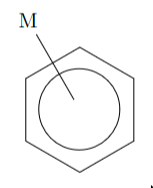
\includegraphics[height=0.20\textwidth]{MBenzene.png}
    \captionof{figure}{$M^{2+}-C_6H_6$}
\end{center}

Se estudiarán las distancias de enlace, cargas de Mulliken y frecuencias de vibración del enlace metal-anillo para M=Be, Mg, Ca y Sr

\subsection{Base 6-31G y LANL2DZ para Sr}

\begin{table}[H]
    \centering
    \begin{tabular}{rccccc}
        \hline
        M  & $d_{M-ring}/\r{A}$ & $d_{C-C}/\r{A}$ & $d_{C-H}/\r{A}$ & $q_{M}$ & $\nu_{M-ring}/cm^{-1}$ \\
        \hline
        -  & -               & 1.3885          & 1.0732          & -       & -               \\
        Be & 1.4042          & 1.4160          & 1.0736          & 0.952   & 615             \\
        Mg & 2.1852          & 1.4105          & 1.0732          & 1.374   & 354              \\
        Ca & 2.7216          & 1.4019          & 1.0735          & 1.723   & 227              \\
        Sr (LANL2DZ) & 2.9796          & 1.4050          & 1.0722          & 1.887   & 155              \\
        \hline
    \end{tabular}
    \caption{Distancias de enlace, carga (Mulliken) y frecuencia de vibración de compuestos $M^{2+}-C_6H_6$, base 6-31G(d)}
\end{table}

La distancia del enlace Metal-anillo aumenta con el tamaño del átomo.
La distancia de enlace C-C y C-H, se mantienen relativamente constantes, pero si varían un poco, ya que los carbonos toman una carga negativa, para compensar la carga positiva del metal, y los hidrógenos toman una carga positiva, por estar enlazados a los carbonos. Por esto, la distancia de enlace C-C aumenta ligeramente, ya que los carbonos tienen carga de igual signo (-), y la distancia de enlace C-H disminuye ligeramente, ya que los hidrógenos (+) se acercan a los carbonos (-).

La carga del metal, aumenta con el tamaño del átomo, son más electropositivos, y más polarizables, con una mayor capacidad de aceptar electrones.

Por ultimo, la frecuencia de vibración del enlace metal-anillo, disminuye con el tamaño del átomo, ya que la masa reducida del sistema aumenta, y la constante de fuerza del enlace disminuye, al aumentar la distancia de enlace.

\subsection{Base 6-31G(d)}
\begin{table}[H]
    \centering
    \begin{tabular}{rccccc}
        \hline
        M  & $d_{M-ring}/\r{A}$ & $d_{C-C}/\r{A}$ & $d_{C-H}/\r{A}$ & $q_{M}$ & $\nu_{M-ring}/cm^{-1}$ \\
        \hline
        -  & -               & 1.3885          & 1.0732          & -       & -               \\
        Be & 1.3315          & 1.4108          & 1.0768          & 0.626   & 641             \\
        Mg & 1.9924          & 1.4071          & 1.0759          & 1.019   & 365             \\
        Ca & 2.5202          & 1.3998          & 1.0756          & 1.577   & 253             \\
        \hline
    \end{tabular}
    \caption{Distancias de enlace, carga (Mulliken) y frecuencia de vibración de compuestos $M^{2+}-C_6H_6$, base 6-31G(d)}
\end{table}

Las conclusiones sacadas entre los distintos metales, son iguales a las sacadas con la base 6-31G.

Comparando la base 6-31G con la base 6-31G(d), se observa que la carga del metal disminuye al añadir orbitales de polarización a la base, ya que la base 6-31G da una descripción demasiado iónica. 

Las distancia de enlace Metal-Benzeno son ligeramente menores con la base 6-31G(d), algo que va al contrario de lo que cabria esperar por la diferencia de cargas. Esto se debe a que la constante de fuerza aumenta, porque aumenta el carácter covalente del enlace, que fortalece la interacción metal-anillo.




\newpage

\begin{thebibliography}{9}
\bibitem{batista_gaussian}
Batista, V. S. \emph{Effective Core Potential (ECP) Basis Sets} 

Disponible en línea: \url{https://batistalab.com/classes/tutorials/gaussian/ECP_bases.pdf} 

\bibitem{atkins_mqm}
Atkins, P. W.; Friedman, R. \emph{Molecular Quantum Mechanics}; 5th ed.; Oxford University Press: Oxford, 2010.

\bibitem{marquez_sn2h4}
Márquez, A.; González, G. G.; Fernández Sanz, J. \emph{Ab-initio calculations on the molecular structure of Sn\textsubscript{2}H\textsubscript{4}}. Chemical Physics, \textbf{138} (1989) 99–104. North-Holland, Amsterdam.




\end{thebibliography}

\end{document}
:\While{}
    \State 
\EndWhile

